\documentclass{article}
\usepackage{graphicx}
\usepackage{ragged2e}
\usepackage{geometry}
\title{Experimentation}
\author{Vigneswaran Chandrasekaran}
\date{10-11-2019}

\begin{document}
\subsection{Comparison with other Pre-training techniques}
The proposed bin-wise pre-training model was compared with the existing pre-training
models: Stacked Autoencoders and Supervised Greedy layer-wise pre-training model.
Stacked Autoencoder was configured with three stacks of encoder-decoder, whereas
Supervised Greedy layer-wise pre-training model was shaped with six layers added
sequentially.
\\
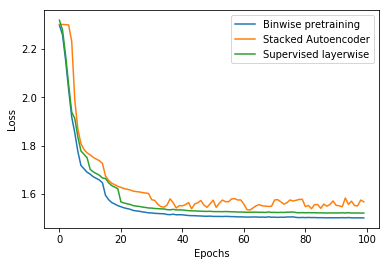
\includegraphics[width= 7cm, height=5cm]{fig7.png}
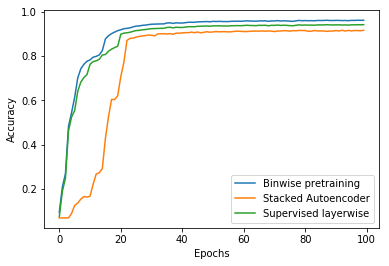
\includegraphics[width= 7cm, height=5cm]{fig8.png}
\\
Fig 10(a) \& Fig 10(b) shows the validation loss and Validation accuracy of Pretraining methods for MNIST dataset respectively
\\
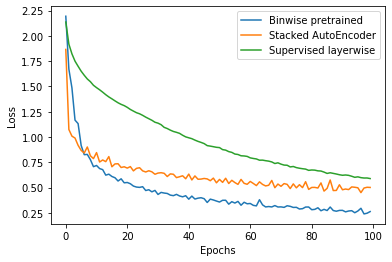
\includegraphics[width= 7cm, height=5cm]{fig9.png}
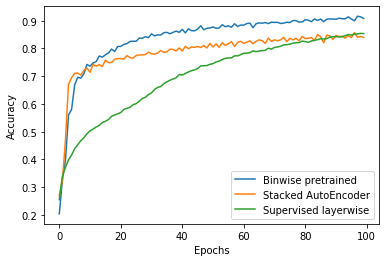
\includegraphics[width= 7cm, height=5cm]{fig10.png}
\\
Fig 11(a) \& Fig 11(b) depicts the validation loss and Validation accuracy of Pretraining methods for Fashion MNIST dataset respectively
\\
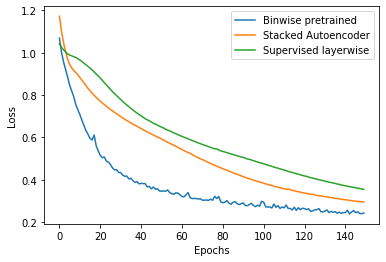
\includegraphics[width= 7cm, height=5cm]{fig11.png}
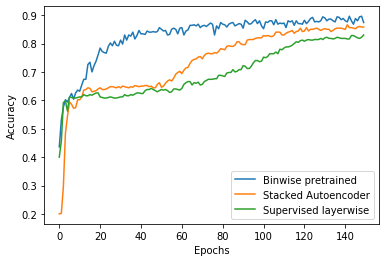
\includegraphics[width= 7cm, height=5cm]{fig12.png}
Fig 12(a) \& Fig 12(b) plots the validation loss and Validation accuracy of various Pretraining methods for University of Bern EEG dataset respectively

\subsection{Regularization Capability}
To evaluate the performance of the proposed work in Regularization perspective, the
distribution of randomly initialized weights and weights after bin-wise pre-training
were recorded and the change imbibed on them due to bin-wise pre-training were
analysed. It was inferred that the weight boundaries were maintained within 0.04 and
the variance of both the distribution remains the same throughout the pre-training
process which confirms that the proposed model behaves as a good regularizer. Fig. 13.
shows the comparison of distribution of randomly initialized weights and pre-trained
weights. Fig. 14. depicts the pattern of weight updation during pre-training process and
it was inferred that the new weights obtained had the desirable distribution, thus
making the Deep Learning model simple with better Generalization behaviour along
with less susceptible to overfitting and Vanishing or Exploding gradient problems.
\\
\\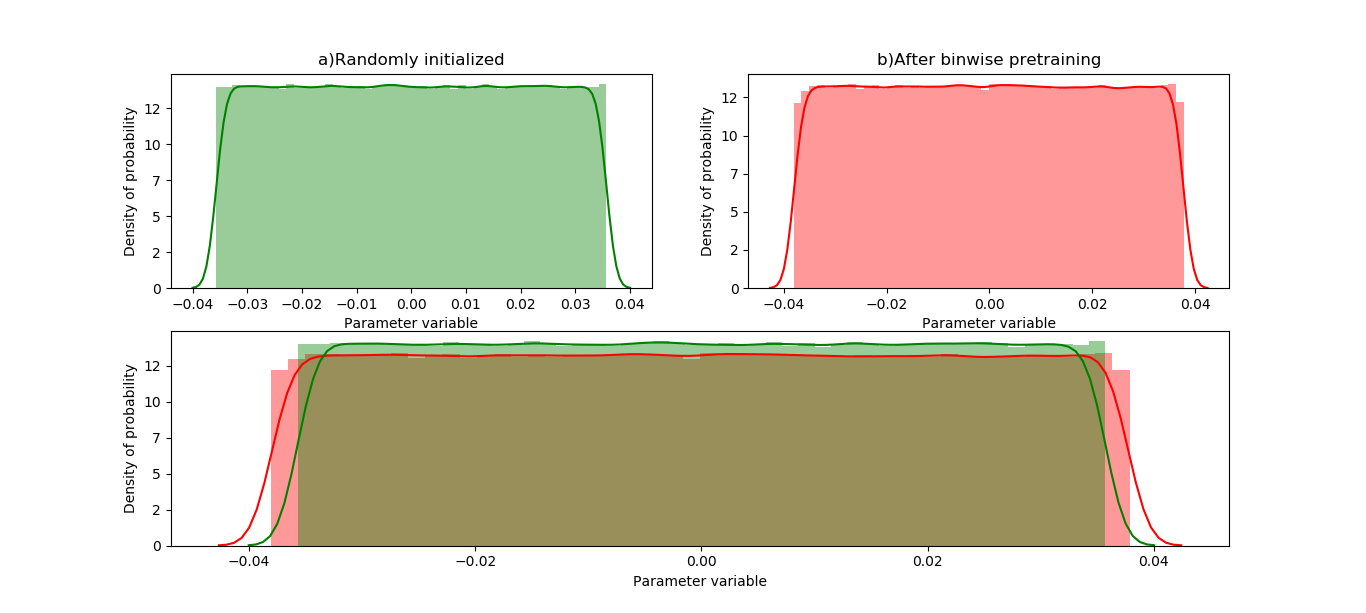
\includegraphics[width= 15cm, height=8cm]{fig13.png}
\\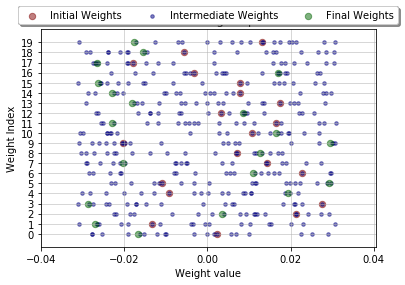
\includegraphics[width= 15cm, height=8cm]{fig14.png}
\\
Fig. 14. Weight updation pattern of randomly selected twenty weights for twenty
iterations during pre-training process.
\\
\subsection{Convergence Rate}
Rate of convergence is an important metric that measures the ability of the model to
converge in better minima with reasonable amount of time. From Fig. 7, 8 \& 9 it has
been inferred that the rate of convergence for all the existing approaches were mostly
similar at the beginning and as the iteration proceeded the proposed unsupervised bin-
wise pre-training model converges earlier than others. Selecting appropriate number of
bins using Partial Information Decomposition alters the degree of change and directly
influences the convergence rate. Fig. 15. shows the increase in Mutual Information
between Neuron’s output ( ) and Input data ( ) as the iterations were proceeded.
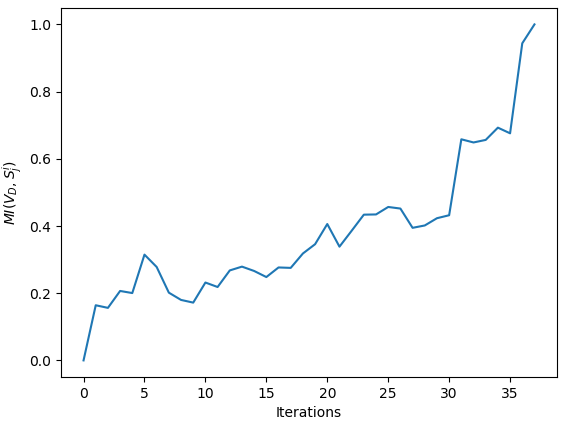
\includegraphics[width=14cm, height=6cm]{fig15}

\end{document}

